% =====================================================================
%  Trained on a judge, tested by another
%  PTO vs GRPO for Motivational Interviewing at matched look-ahead (K=0)
%  Target: CLPsych / NLP-for-psychology workshop (ACL style)
% =====================================================================
%
% COMPILING
%   This file is written for the official ACL style (`acl.sty` + `acl_natbib.bst`),
%   which is NOT vendored here. Two ways to build:
%     (a) Overleaf -> "ACL (ARR) template" -> drop these files in. Recommended.
%     (b) Locally, after copying acl.sty / acl_natbib.bst next to this file.
%   Without acl.sty the preamble falls back to a plain single-column article so
%   the draft still compiles for reading. Line counts will not match the venue.
%
\documentclass[11pt]{article}

\IfFileExists{acl.sty}{%
  \usepackage[review]{acl}      % swap to [] for the camera-ready
}{%
  \usepackage[margin=1in]{geometry}
  \usepackage{natbib}
  \bibliographystyle{plainnat}
  \typeout{^^J*** acl.sty not found - building in FALLBACK single-column mode. ***^^J}
}

\usepackage{times}             % REQUIRED: scalable Type 1 fonts. Without this,
\usepackage{latexsym}          % microtype's font expansion fails on bitmap CM.
\usepackage[T1]{fontenc}
\usepackage[utf8]{inputenc}
\usepackage{microtype}
\usepackage{graphicx}
\usepackage{booktabs}
\usepackage{multirow}
\usepackage{amsmath}
\usepackage{amssymb}
\usepackage{xcolor}
\usepackage{pifont}            % \ding{55} = the MITI "below threshold" mark
\usepackage[normalem]{ulem}

% --- draft aids: \todo{...} and \note{...} vanish when \draftfalse -------------
\newif\ifdraft\drafttrue
\ifdraft
  \newcommand{\todo}[1]{\textcolor{red}{\textbf{[TODO: #1]}}}
  \newcommand{\note}[1]{\textcolor{blue}{\textit{[#1]}}}
\else
  \newcommand{\todo}[1]{}
  \newcommand{\note}[1]{}
\fi

% --- shorthands ---------------------------------------------------------------
\newcommand{\QQ}{Q1{+}Q2}
\newcommand{\mici}{MICI}
\newcommand{\dz}{\ensuremath{d_z}}
\newcommand{\primaryjudge}{\textsc{gpt-4o-mini}}
\newcommand{\heldoutjudge}{\textsc{Claude Haiku 4.5}}

\title{Trained on a Judge, Tested by Another: Exploration Beats Group-Relative
Optimization When the Reward Is a Questionnaire-Filling LLM}

% \todo{confirm author list + order with Kfir/Doron before submission}
\author{
  Lior Baruch \\
  School of Computer Science \\
  Reichman University, Herzliya, Israel \\
  \texttt{lior95bar@gmail.com}
  \\[1ex]
  \todo{co-authors: Kfir Bar, Doron Friedman, Moshe Butman?}
}

\begin{document}
\maketitle

% !TeX root = ../main.tex
\begin{abstract}
Small language models can be trained to conduct Motivational Interviewing (MI) by
simulating sessions against an LLM patient and rewarding them with an LLM that fills in
validated MI questionnaires. We ask what such training actually buys. Holding the base
model (Llama-3.2-1B), the patient simulator, the grading oracle, the candidate budget and
the look-ahead depth fixed, we compare two ways of turning the same reward into a policy
update over ten iterations: Preference-Tree Optimization (PTO), which grows a sequential
search over therapist turns and trains with DPO on the surviving pairs, and Group-Relative
Policy Optimization (GRPO), which trains on standardized advantages over a group of
completions. Every model state is evaluated on 96 patient personas across eight
instruments.
%
Both methods improve substantially on the rubric they optimize, but PTO leads at the
matched ten-iteration endpoint (\QQ{} $4.26$ vs $3.75$; paired $+0.51$, $\dz{}=0.73$),
because GRPO peaks at iteration~8 and then regresses. The gains arrive with a measurable
drift toward affirmation: literal question rates fall from $0.83$ to $0.15$ per therapist
turn in GRPO, and MI-inconsistent behaviour rises ${\sim}2.3\times$ (PTO) and
${\sim}4\times$ (GRPO).
%
Re-scoring all $22{,}272$ conversation$\times$rubric cells with a held-out judge from a
different model family preserves $88.3\%$ of contrast signs ($98.9\%$ at
$|\Delta|\!\ge\!0.50$), but separates the arms on \emph{gain retention}: the fraction of
each arm's Q1 gain the held-out judge still credits diverges from iteration~3 onward,
ending at $0.80$ for PTO and $0.28$ for GRPO. Finally, reading the training signal
directly shows the difference is a property of the \emph{data} the two methods collect,
not of their losses. We argue that questionnaire-filling LLM judges should be treated as
optimization targets that must themselves be audited, and that gain retention under a
decoupled grader is a cheap, general test for doing so.
\end{abstract}

% !TeX root = ../main.tex
\section{Introduction}
\label{sec:intro}

Motivational Interviewing \citep[MI;][]{miller1991mi} is a counselling style for helping
people resolve ambivalence about change. It is defined less by what the counsellor says
than by how they say it: open questions, reflective listening, affirmation of the client's
own strengths, and a studied refusal to argue for change on the client's behalf. That
makes MI an attractive and unusually demanding target for goal-oriented dialogue systems.
The behaviour to be learned is multi-turn, the reward is delayed, and expert-annotated
data is scarce and expensive.

The now-standard workaround is to close the loop with language models: a large model plays
the patient, another large model plays an evaluator that fills in validated MI
questionnaires, and a small model is trained against the resulting score
\citep{yosef2024assessing, baruch2025pto}. This is attractive because it is cheap and
because the questionnaires are instruments clinical researchers already trust. It is also
a reward-model design in which the reward model is a black box that was never trained to
be robust to optimization pressure --- and the training loop pushes on it for ten
iterations.

This paper asks two questions about that loop, and answers them under tightly matched
conditions. First: \textbf{how should the reward be turned into a policy update?} We compare
Preference-Tree Optimization (PTO), which grows a \emph{sequential} search over therapist
turns and trains with DPO \citep{rafailov2023dpo} on the surviving preference pairs,
against Group-Relative Policy Optimization \citep[GRPO;][]{shao2024deepseekmath}, which
samples an i.i.d.\ group of completions per prompt and trains on standardized advantages.
Second: \textbf{what do the resulting gains mean?} A questionnaire score that goes up is a
claim about the therapist only to the extent that the questionnaire-filler is not being
gamed.

We hold everything except the two answers fixed: the same Llama-3.2-1B base policy, the
same simulated patients, the same \primaryjudge{} oracle and reward composition, the same
per-prompt candidate budget ($M = G = 8$), the same minimum-context filter, and the same
look-ahead depth ($K=0$). Both arms run ten iterations, regenerating their training data
from the current policy each time; each of the 22 resulting model states is evaluated on
96 patient personas and scored on eight instruments --- five global rubrics, a patient
change-talk coder, an MI-inconsistency coder, and the MITI technique ratios.

\paragraph{Contributions.}
\begin{enumerate}\itemsep2pt
  \item \textbf{A matched comparison of preference-tree and group-relative optimization
  for MI.} Both methods produce large gains over the base policy; PTO leads at the matched
  ten-iteration endpoint (\QQ{} $4.26$ vs $3.75$; paired $+0.51$, $\dz{}=0.73$,
  Holm $p<0.001$) and climbs monotonically, whereas GRPO peaks at iteration~8 and regresses
  (\S\ref{sec:results}).

  \item \textbf{A characterisation of what the reward actually purchases.} In both arms the
  therapist drifts toward affirmation and away from inquiry --- affirmations per turn rise
  ${\sim}5\times$ while literal question rates fall --- and MI-inconsistency rises with the
  scores it is supposed to contradict. We trace this to specific items of the reward
  questionnaire, not only to the optimizer (\S\ref{sec:hacking}).

  \item \textbf{Gain retention under a decoupled judge as a reward-hacking test.} We
  re-score every conversation with a judge from a different model family that never played
  the patient and never touched training. Contrast signs survive ($88.3\%$ overall,
  $98.9\%$ at $|\Delta|\!\ge\!0.50$), but the \emph{share of each arm's gain the held-out
  judge still credits} does not: it is an onset curve that separates the arms from
  iteration~3 and ends at $0.80$ (PTO) versus $0.28$ (GRPO). This is a cheap, general
  diagnostic for any LLM-judge-trained system (\S\ref{sec:validity}).

  \item \textbf{Evidence that the method gap is about exploration, not the loss.} Putting
  both methods' updates on one probe, swapping the weighting rule on the \emph{same}
  candidate groups barely moves the update direction, while holding the rule fixed across
  each method's \emph{own} groups leaves them as far apart as when trained
  (\S\ref{sec:mechanism}; full construction and per-iteration series in
  Appendix~\ref{app:mechanism}).
\end{enumerate}

The practical reading for the CLPsych community is deflationary and, we think, useful: with
an LLM oracle in the loop, ``all rubrics went up'' is not evidence of clinical skill, and
the difference between two RL algorithms may be a difference in what conversations they
bother to look at.

% !TeX root = ../main.tex
\section{Background and Related Work}
\label{sec:related}

\paragraph{MI and simulated clients.}
Because MI sessions are confidential and expert coding is slow, work on computational MI
has increasingly used LLM-simulated clients as both a training environment and an
evaluation harness. \citet{yosef2024assessing} showed that an LLM prompted with the
session-satisfaction and working-alliance instruments used here produces ratings that are
statistically reliable and that separate three levels of therapist expertise --- the
validation basis on which those two instruments are used as an LLM evaluator, and the
reason we treat them as a satisfaction/alliance proxy rather than as clinical outcome
measures. \todo{cite 1--2 more recent MI-simulation papers (2025--2026) so this does not
read as lab-internal; check \citet{steenstra2024scaffolding}-style work and MI-coding LLM
papers.}

\paragraph{Preference optimization from self-generated data.}
DPO \citep{rafailov2023dpo} removed the explicit reward model from RLHF
\citep{christiano2017deeprl, ouyang2022instructgpt} and made it practical to train on
preference pairs produced by the model itself and labelled by an automatic judge
\citep{yuan2024selfrewarding, guo2024oaif, pace2024westofn}. Where the pairs come from
matters as much as the loss: search-based construction --- MCTS over reasoning traces
\citep{xie2024mctsdpo}, preference trees \citep{yuan2024eurus}, and dialogue-policy
planning \citep{yu2023promptmcts, chen2025broaden} --- consistently beats i.i.d.\ sampling
in domains where the payoff is delayed. PTO \citep{baruch2025pto} is the MI instance of
this idea: it grows a preference tree over therapist turns and scores each branch after
$K$ further simulated turns, so a candidate is judged by where it \emph{leads} rather than
by how it \emph{looks}. That work established PTO against an untrained baseline; it did not
compare it to an on-policy RL alternative, which is what we do here.

\paragraph{Group-relative optimization.}
GRPO \citep{shao2024deepseekmath} replaces the learned value function of PPO
\citep{schulman2017ppo} with a group baseline: sample $G$ completions for a prompt, and
weight each one's gradient by its reward standardized within the group. It has become the
default recipe for verifiable-reward domains, which makes ``does it transfer to a soft,
LLM-judged, multi-turn domain?'' the natural question --- and one that has to be asked at a
\emph{matched} candidate budget, since PTO's $M$ branches and GRPO's $G$ completions are
the same expenditure of generation and grading.

\paragraph{Reward hacking and LLM judges.}
Optimizing against a learned or prompted evaluator invites the policy to exploit the
evaluator rather than the task \citep{gao2023scaling, skalse2022defining}. In the RLHF
setting the best-documented instance is sycophancy \citep{sharma2024sycophancy,
perez2023discovering}, and LLM judges are known to prefer longer, more assertive and
more flattering answers \citep{zheng2023judging, dubois2024lengthcontrolled}. MI is an
unusually sharp test case for this, because the failure mode has a \emph{clinical} name:
an MI session in which the counsellor praises the client and stops asking questions is not
merely a worse answer, it is MI-inconsistent practice as the MITI manual
\citep{moyers2016miti} defines it. Our contribution here is less the observation that this
happens than the measurement: we quantify it on an instrument outside the reward
(\S\ref{sec:hacking}) and, more sharply, as a train/test generalization ratio across
graders (\S\ref{sec:validity}).

\paragraph{Judge reliability.}
Single-judge evaluation is now routinely criticised for exactly the coupling we have here
--- the same model family generates and grades \citep{panickssery2024selfpreference}. The
standard mitigations are multiple judges and human spot-checks. We report the reliability
of both graders explicitly (ICC over repeated scorings) so that cross-judge agreement can
be read against an attenuation ceiling rather than against $1.0$, which is what makes the
one rubric that genuinely disagrees (MITI) distinguishable from the ones that are merely
noisy.

% !TeX root = ../main.tex
\section{Two Ways to Spend the Same Budget}
\label{sec:method}

Both methods are \emph{iterative}: at each iteration the current policy regenerates its own
training data, an update is applied, the adapter is swapped in, and the loop repeats. They
share the conversation simulator, the oracle, and the look-ahead subroutine, and differ
only in (i)~how rollouts become training data and (ii)~which loss consumes it. This section
fixes notation and states the difference precisely; Figure~\ref{fig:method} draws it.

\paragraph{Notation.}
$\pi_n$ is the therapist policy at the start of iteration $n$ (a LoRA adapter over a frozen
base; $\pi_0$ is the base model). $P$ is the simulated patient, conditioned on one of 96
persona prompts. $O$ is the oracle: it reads a full transcript, fills in the reward
questionnaires under a constrained JSON schema, and returns the mean item score.
$\mathrm{MCL}$ is a floor on how much conversation must precede a training context, and
$K$ is the look-ahead depth.

\paragraph{$K$-turn look-ahead (shared).}
Given a prefix $c$ ending on a patient turn and a candidate therapist completion $t$, the
scored object is not $c\!+\!t$ but the trajectory obtained by simulating $K$ further
alternating turns under the current policy,
\[
  c + t + P(\cdot) + \pi_n(\cdot) + \cdots ,
\]
so that a candidate is rewarded for where it leads rather than for how it reads in
isolation. Both methods call the identical subroutine. \textbf{In this paper $K=0$
throughout}, i.e.\ look-ahead is disabled in both arms; it is the controlled variable of a
companion study and is held at zero here so that the PTO-vs-GRPO contrast is not confounded
with it.

\paragraph{PTO: sequential search, pairwise loss.}
At the start of iteration $n$, $\pi_n$ simulates 96 full conversations. Each is truncated to
its first $\mathrm{MCL}$ utterances to seed a \emph{trunk}. The trunk is then grown one
therapist turn at a time: sample $M$ candidate completions, roll each forward $K$ turns,
score each with $O$, \emph{append the best candidate to the trunk}, let $P$ reply, repeat.
At every branch point, the (best, worst) pair is emitted as a preference pair --- but only
if the score gap exceeds a threshold $\tau$; otherwise the branch point contributes no
training data at all. The collected pairs train a DPO objective against the iteration-start
adapter as reference: writing
$h(y) = \log\frac{\pi(y \mid x)}{\pi_{\mathrm{ref}}(y \mid x)}$ for the log-ratio of a
completion under the policy and the reference,
\[
  \mathcal{L} = -\,\mathbb{E}\big[\log \sigma\big(\beta\,(h(y_w) - h(y_l))\big)\big].
\]
The essential property is that \emph{the winner is fed back}: each choice conditions the
next branch point, so the tree explores states the policy would reach only by making a
sequence of good choices.

\paragraph{GRPO: i.i.d.\ groups, group-relative weights.}
At the start of iteration $n$, $\pi_n$ simulates the same 96 conversations. Every patient
turn whose conversation-so-far is at least $\mathrm{MCL}$ utterances long is sliced off as a
training prompt, and the prompt list is then \emph{fixed} for the iteration. For each
prompt the trainer samples $G$ completions, scores each with $O$ (after the same $K$-turn
roll-forward), and forms the group-relative advantage
$A_g = (r_g - \mathrm{mean}_g\,r)/\mathrm{std}_g\,r$, which weights that completion's
gradient in a PPO-style clipped objective with a KL penalty to the iteration-start
reference. Every completion contributes; there is no threshold and no trunk to advance.

\begin{figure}[t]
  \centering
  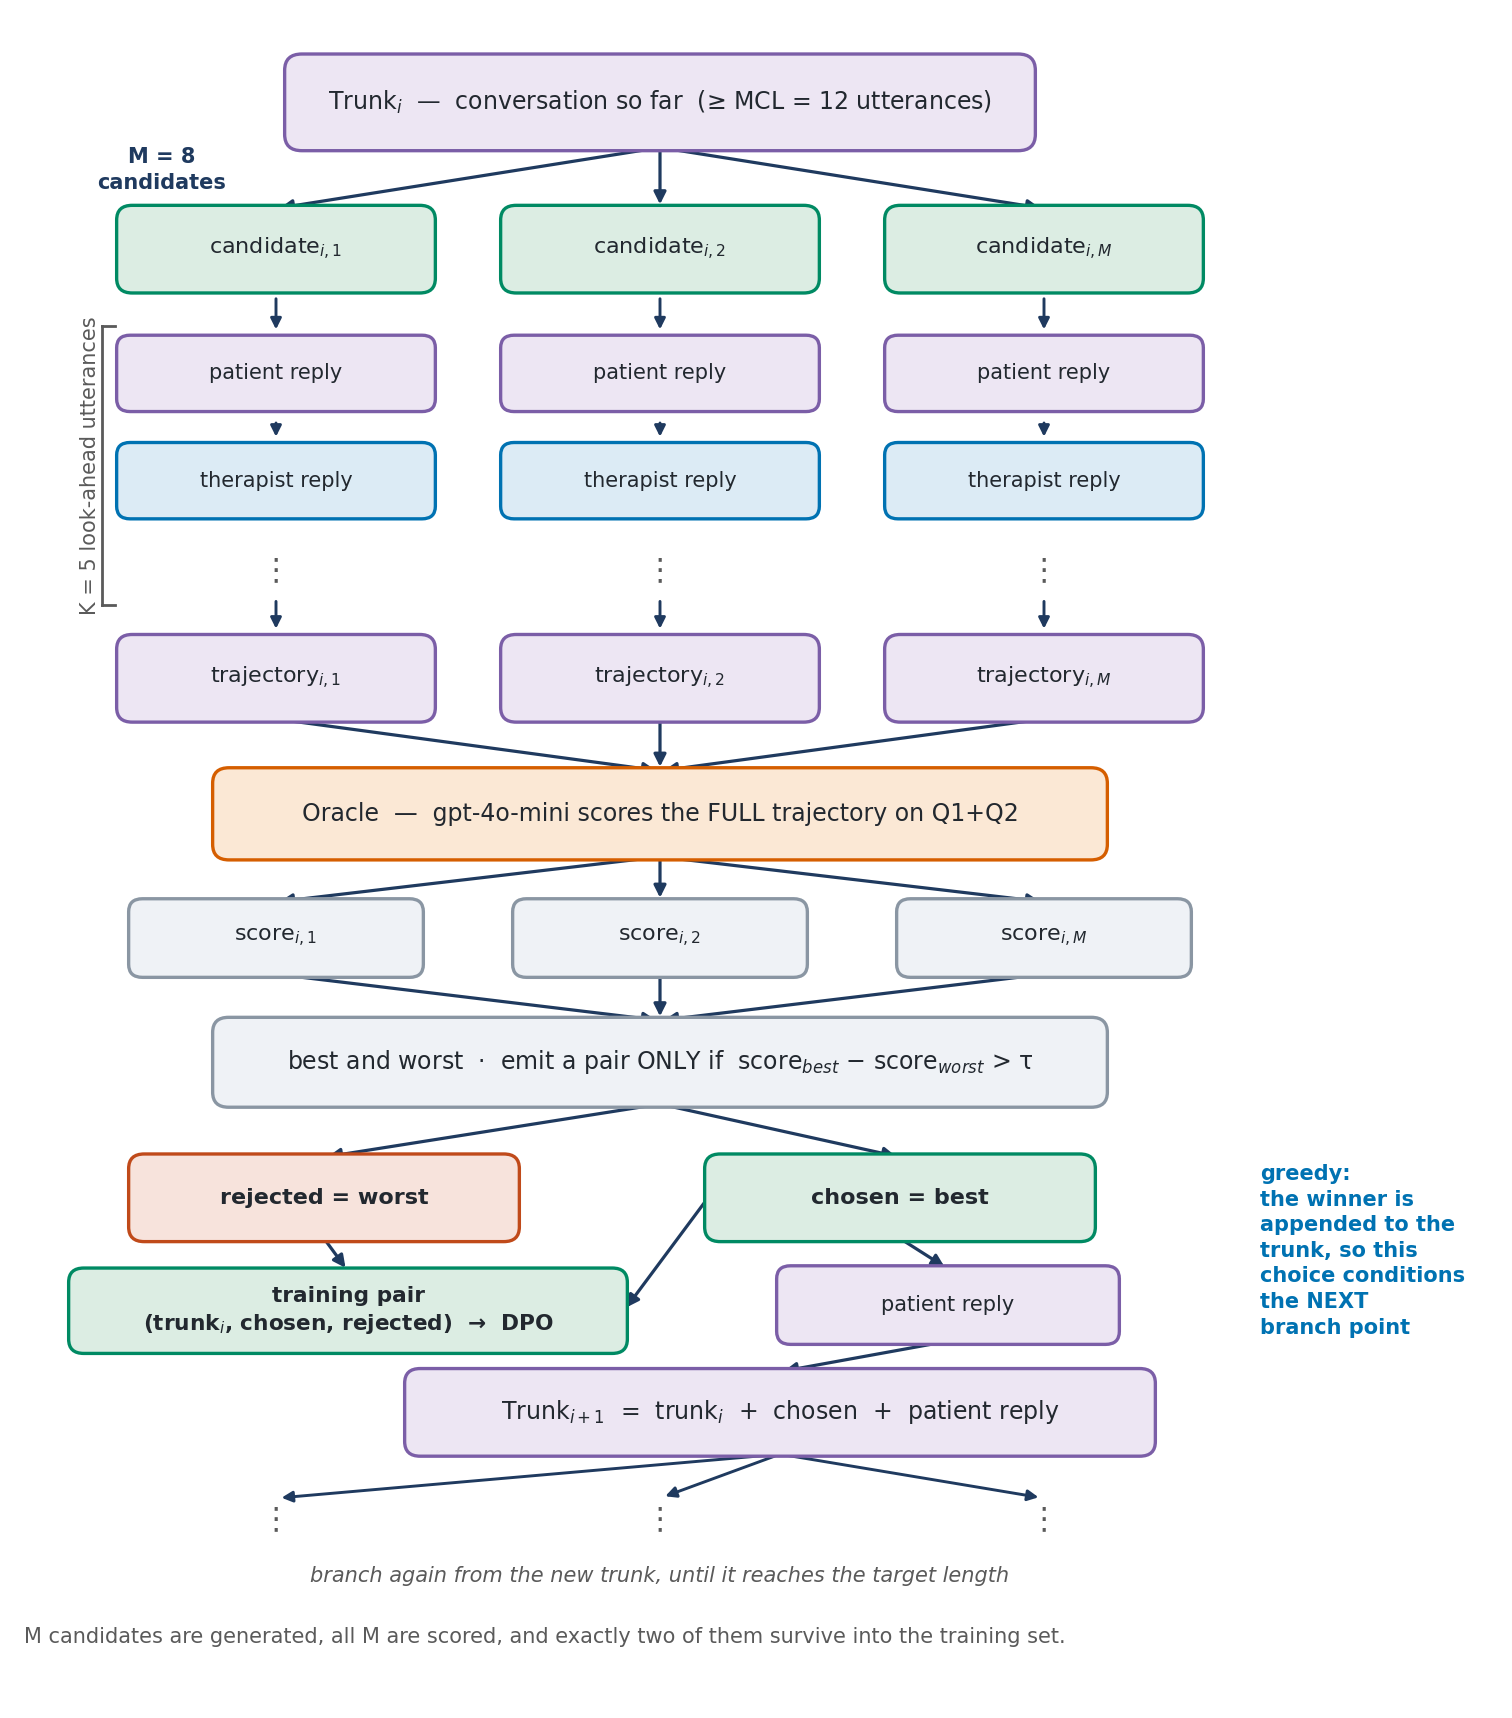
\includegraphics[width=\linewidth]{figures/method_pto_branch.png}\\[4pt]
  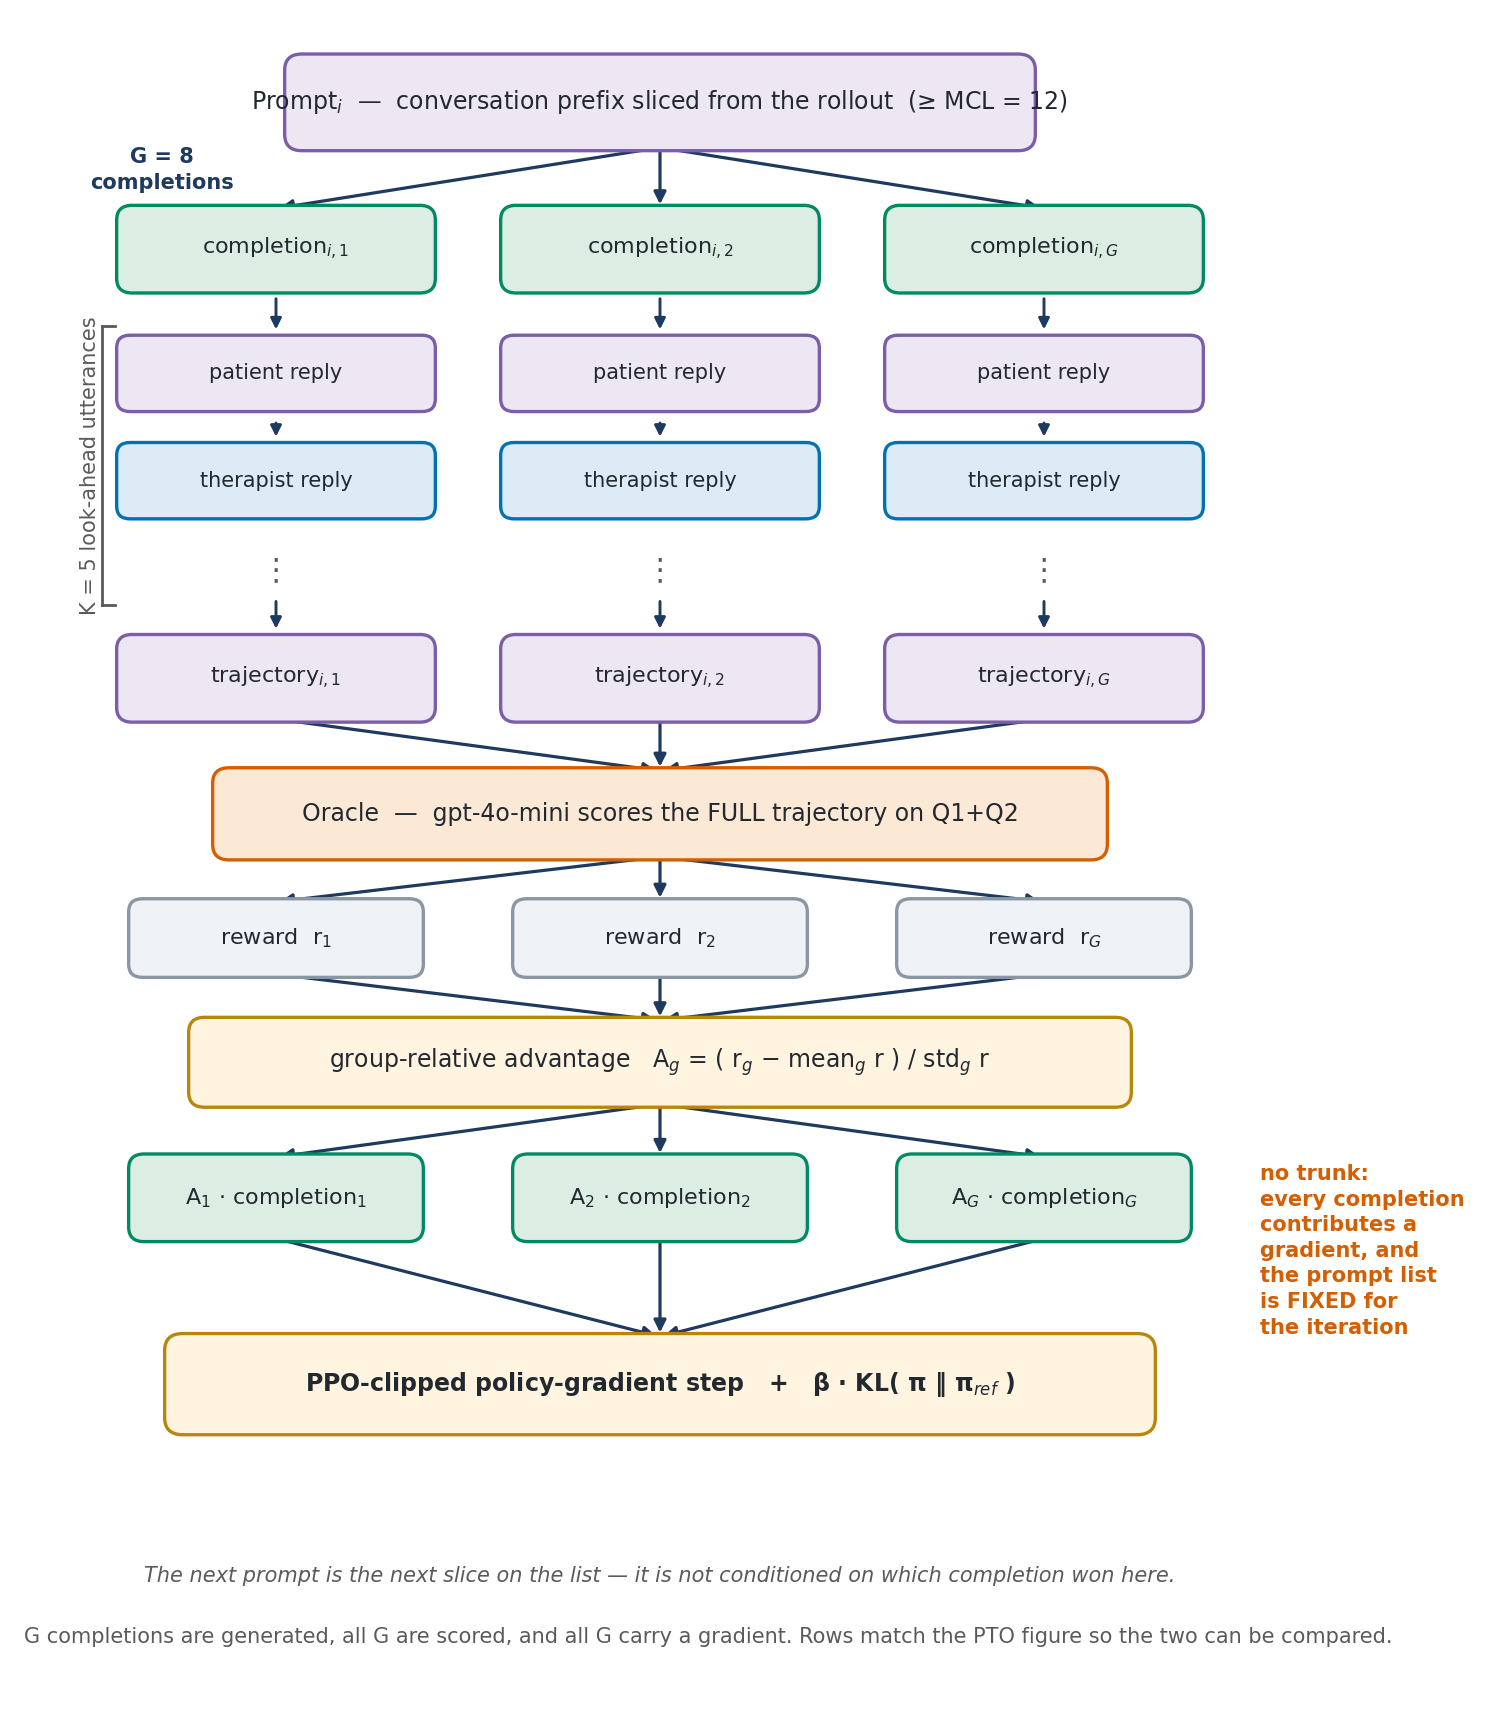
\includegraphics[width=\linewidth]{figures/method_grpo_group.png}
  \caption{One branch point (top, PTO) and one group (bottom, GRPO), drawn on the same row
  grid. Everything above the oracle is identical: same policy, same $M\!=\!G$ samples, same
  $K$-turn roll-forward, same full-trajectory scoring. The methods diverge only in what
  happens to the scores --- PTO keeps exactly two candidates and only when they differ by
  more than $\tau$, then appends the winner to the trunk; GRPO gives all $G$ a gradient
  weight and discards the rollout. The diagrams are drawn at $K\!=\!5$; this paper's
  experiments use $K\!=\!0$.}
  \label{fig:method}
\end{figure}

\paragraph{What is matched, and what is not.}
Table~\ref{tab:matched} lists the controlled variables. The two methods spend the same
number of policy samples per decision point ($M = G = 8$) against the same oracle, so the
comparison is not one of compute at the candidate level. What is deliberately \emph{not}
matched is what those samples are spent on --- and that, we argue in
\S\ref{sec:mechanism}, is where the difference lives. Two further asymmetries follow from
the designs themselves and are reported rather than corrected: PTO discards a branch point
whose candidates tie within $\tau$ (GRPO discards nothing), and PTO's trunk visits states
that GRPO's fixed prompt list never contains.

% !TeX root = ../main.tex
\section{Experimental Setup}
\label{sec:setup}

\paragraph{Models.}
The therapist is \texttt{Llama-3.2-1B} in \texttt{bfloat16} with a LoRA adapter
($r{=}16$, $\alpha{=}16$, dropout $0.05$, applied to all attention and MLP projections).
The patient simulator and the training oracle are both
\texttt{gpt-4o-mini-2024-07-18}; the oracle answers under a constrained JSON schema.
Using a 1B policy is a deliberate constraint, not a convenience: it is the regime in
which an institution could plausibly run a therapist model locally, and it is the regime in
which reward-hacking is most visible because the policy has the least capability to spend
on anything else.

\paragraph{Patients.}
96 patient personas enumerate a full factorial over gender ($2$) $\times$ cooperation level
($3$: low, high, low-then-rising) $\times$ presenting problem ($2$: smoking, obesity)
$\times$ problem duration ($2$) $\times$ prior quit attempts ($2$) $\times$ age
($2$: 27, 61). The therapist persona is held fixed at the ``expert'' level. Personas are
shuffled between iterations; because the same 96 personas recur at every model state, all
comparisons in this paper are \textbf{persona-paired} ($n{=}96$).

\paragraph{Training configuration (matched).}
Table~\ref{tab:matched} gives the controlled variables. Both arms run
$10$ iterations, $2$ epochs per iteration, regenerating 96 conversations per iteration
from the current policy, with a training-context floor of $\mathrm{MCL}=12$ utterances,
$M = G = 8$ candidates per decision point, candidate sampling temperature $1.2$, generation
temperatures $0.9$ (therapist) / $0.7$ (patient), a $200$-token completion cap, and
learning rate $10^{-5}$. Method-specific: PTO uses $\tau=0.1$ and DPO
$\beta=0.1$ (sigmoid loss); GRPO uses a KL coefficient of $0.01$.

\begin{table}[t]
  \centering\small
  \begin{tabular}{@{}ll@{}}
    \toprule
    \multicolumn{2}{@{}l}{\textbf{Matched across both arms}}\\
    \midrule
    Base policy        & Llama-3.2-1B, bf16, LoRA $r{=}16$\\
    Patient / oracle   & \texttt{gpt-4o-mini-2024-07-18}\\
    Training reward    & mean(Q1, Q2), 22 items\\
    Iterations         & 10 ($\times$ 2 epochs)\\
    Convs / iteration  & 96 (one per persona)\\
    Candidates / point & $M = G = 8$ @ temp.\ $1.2$\\
    Look-ahead         & $K = 0$\\
    Context floor      & $\mathrm{MCL} = 12$ utterances\\
    Learning rate      & $1\!\times\!10^{-5}$\\
    \midrule
    \multicolumn{2}{@{}l}{\textbf{Method-specific}}\\
    \midrule
    PTO                & $\tau = 0.1$, DPO $\beta = 0.1$\\
    GRPO               & KL $\beta = 0.01$, all $G$ kept\\
    \bottomrule
  \end{tabular}
  \caption{Controlled variables. The two arms differ in how rollouts become training data
  and in the loss, not in generation budget or grading.}
  \label{tab:matched}
\end{table}

\paragraph{Reward vs.\ evaluation.}
The \emph{training} reward is the mean of two instruments only --- Q1 (session
satisfaction, 5 items) and Q2 (working alliance / relational communication, 17 items), the
LLM-evaluator prompts validated by \citet{yosef2024assessing}, matching
\citet{baruch2025pto}. The \emph{evaluation} battery is deliberately wider
(Table~\ref{tab:instruments}): five global rubrics, a patient change-talk coder, an
MI-inconsistency coder, and three MITI technique ratios computed from the coded behaviour
counts. Only \QQ{} is inside the reward; everything else is an outside-the-reward axis, and
we flag which is which throughout.

\begin{table}[t]
  \centering\small
  \setlength{\tabcolsep}{4pt}
  \begin{tabular}{@{}llc@{}}
    \toprule
    Instrument & What it rates & Reward?\\
    \midrule
    \QQ{}       & satisfaction + alliance   & \textbf{yes}\\
    WAI-SR      & alliance: goal/task/bond  & no\\
    CSQ-8       & client satisfaction       & no\\
    MI-SAT      & MI-session satisfaction   & no\\
    MITI        & MI treatment integrity    & no\\
    PCT         & \emph{patient} change-talk & no\\
    \mici{}~$\downarrow$ & MI-\emph{inconsistent} moves & no\\
    R:Q, \%CR, \%MICO & MITI technique ratios & no\\
    \bottomrule
  \end{tabular}
  \caption{The evaluation battery. \mici{} is the only metric where lower is better. WAI-SR
  \citep{hatcher2006waisr} and CSQ-8 \citep{larsen1979csq} are classically validated human
  self-report scales completed by the oracle in the patient's voice; MITI is the official
  coding manual \citep{moyers2016miti}; PCT and \mici{} are MITI-style coders written for
  this study.}
  \label{tab:instruments}
\end{table}

\paragraph{Evaluation protocol.}
The 96 conversations generated at the start of iteration $n$ are the output of the
iteration-$(n\!-\!1)$ policy, so they \emph{are} that policy's evaluation set --- no
separate generation pass is needed for trained states. Every conversation is scored on all
eight instruments at temperature $0.1$ with a fixed seed. Across the two arms this is 22
model states $\times$ 8 rubrics $\times$ 96 conversations. Contrasts are persona-paired
Wilcoxon tests with Holm correction within each family (the eight rubrics of one contrast,
or the ten iterations of one arm-vs-base sweep); effect sizes are $\dz{}$. Confidence
intervals are persona bootstraps at a fixed seed.

\paragraph{Second grader.}
For \S\ref{sec:validity} the entire grid was re-scored by \heldoutjudge{} --- a different
model family that never played the patient and never touched training --- at full coverage
($22{,}272/22{,}272$ cells). The two graders are \textbf{never averaged}: the primary
oracle \emph{was} the training reward and the second was held out, which makes this a
train-vs-test comparison rather than two interchangeable raters, and their level offset
($1.2$--$1.7$ points, and model-dependent) would silently shrink every effect. Only
contrasts and standardized quantities are combined across graders.

% !TeX root = ../main.tex
\section{Both Methods Work; One Keeps Working}
\label{sec:results}

\begin{table*}[t]
  \centering\small
  \begin{tabular}{@{}lrrrrrrrr@{}}
    \toprule
    & \multicolumn{3}{c}{\textbf{PTO}} & \multicolumn{3}{c}{\textbf{GRPO}}
    & \multicolumn{2}{c}{\textbf{PTO $-$ GRPO @10}}\\
    \cmidrule(lr){2-4}\cmidrule(lr){5-7}\cmidrule(lr){8-9}
    Metric & base & @10 & $\dz{}$ & base & @10 & $\dz{}$ & $\Delta$ & $\dz{}$\\
    \midrule
    \QQ{}~\emph{(reward)} & 3.00 & \textbf{4.26} & 1.43 & 3.07 & 3.75 & 0.72 & $+0.51^{***}$ & 0.73\\
    WAI-SR                & 2.85 & 3.50 & 0.97 & 2.89 & 3.44 & 0.84 & $+0.06^{\phantom{***}}$ & 0.12\\
    CSQ-8                 & 2.38 & 2.95 & 0.81 & 2.36 & 2.77 & 0.59 & $+0.17^{*}$   & 0.31\\
    MI-SAT                & 2.84 & 3.65 & 0.90 & 2.86 & 3.48 & 0.66 & $+0.17^{*}$   & 0.27\\
    MITI                  & 3.13 & 4.27 & 1.35 & 3.22 & 3.92 & 0.82 & $+0.35^{***}$ & 0.46\\
    PCT                   & 0.49 & 0.63 & 0.62 & 0.49 & 0.57 & 0.36 & $+0.06^{*}$   & 0.29\\
    \mici{}~$\downarrow$  & 0.21 & \textbf{0.49} & 0.78 & 0.21 & \textbf{0.84} & 1.72 & $-0.35^{***}$ & $-0.99$\\
    \bottomrule
  \end{tabular}
  \caption{Endpoint results at the matched tenth iteration, persona-paired over $n{=}96$.
  Left blocks: each arm's own base and its iteration-10 mean, with the paired $\dz{}$ of the
  gain over base (all Holm $p\!\approx\!0$). Right block: the paired PTO$-$GRPO difference
  at iteration~10 ($^{***}$ Holm $p<0.001$, $^{*}$ $p<0.05$; blank = n.s.). \mici{} is
  MI-\emph{inconsistency}, where lower is better, so its negative difference favours PTO.
  Primary grader (\primaryjudge{}).}
  \label{tab:endpoint}
\end{table*}

\begin{figure}[t]
  \centering
  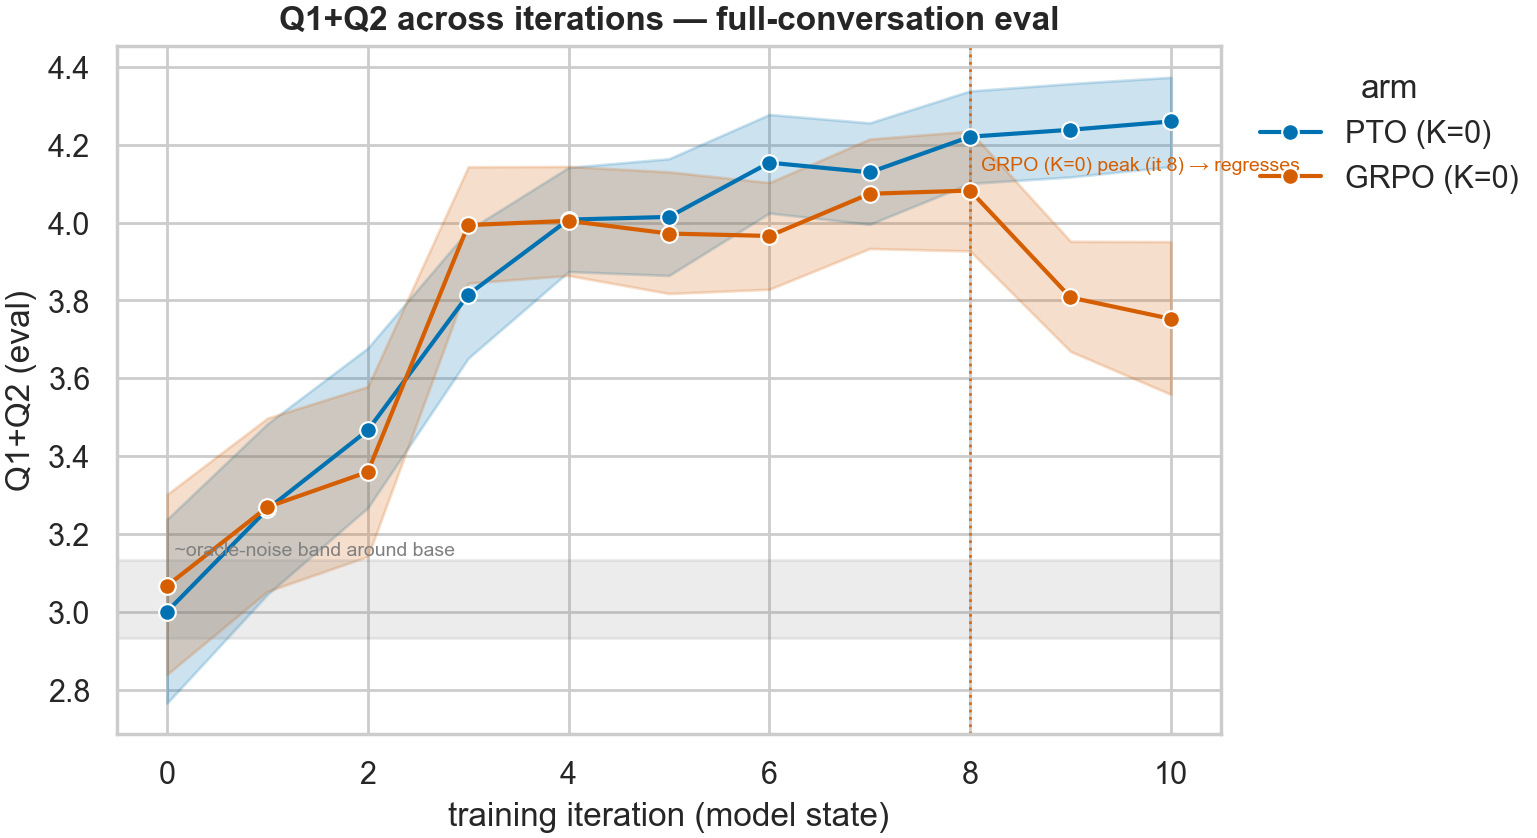
\includegraphics[width=\linewidth]{figures/trajectory_Q1Q2_gpt-4o-mini.png}
  \caption{\QQ{} (the training reward) across iterations, persona-paired means with 95\%
  CIs. PTO climbs monotonically to iteration~10; GRPO peaks at iteration~8 and regresses.
  Primary grader.}
  \label{fig:trajectory}
\end{figure}

\paragraph{Training works, and it works a lot.}
Both arms move the base 1B policy a long way. On the training reward, PTO goes
$3.00 \to 4.26$ ($\dz{}=1.43$) and GRPO $3.07 \to 4.08$ at its peak
($\dz{}=1.22$); every one of the five global rubrics is a large effect for PTO, with
Holm-corrected $p\!\approx\!0$ throughout (Table~\ref{tab:endpoint}). Degeneration is
eliminated: the base policy loops a verbatim therapist turn in $48$--$49\%$ of
conversations, and both arms drive that to $0$ by iteration~10. Sessions also lengthen
substantially per turn --- mean therapist turn length rises from ${\sim}270$--$300$ to
$686$ (PTO) and $896$ (GRPO) characters. Taken alone, this is a success story.

\paragraph{PTO leads at the matched endpoint, because GRPO regresses.}
At iteration~10 the paired difference is $+0.51$ \QQ{} in PTO's favour
($\dz{}=0.73$, Holm $p<0.001$), with MITI, MI-SAT, CSQ-8, PCT and \mici{} also favouring
PTO and only WAI-SR indistinguishable. The reason is visible in
Figure~\ref{fig:trajectory}: the two arms track each other for the first eight iterations
--- at iteration~8 the gap is only $+0.14$ --- and then diverge, because GRPO peaks at
iteration~8 ($4.08$) and falls to $3.75$ while PTO continues to $4.26$. Fitting a line
through each arm's trajectory gives $0.120$ \QQ{}/iteration for PTO against $0.072$ for
GRPO, with PTO's peak at its final iteration and GRPO's four iterations earlier.

We also report the \emph{steelman} comparison, since an experimenter with a validation set
would have stopped GRPO at its peak: PTO@10 still beats GRPO@8 by $+0.18$ \QQ{}
($\dz{}=0.30$, Holm $p=0.010$), along with CSQ-8, MI-SAT, WAI-SR and PCT; MITI and \mici{}
are indistinguishable at that pairing. So the ranking does not depend on GRPO's late
collapse --- but the \emph{size} of the ranking does, and honest reporting of an iterative
method should give both.

\paragraph{An iteration-9 dip, and what it is not.}
GRPO drops sharply at iteration~9 across nearly every metric simultaneously and partially
recovers at~10. We report it rather than smoothing it: it is a single-iteration event on
top of an already-monotonic decline from the iteration-8 peak, and \S\ref{sec:mechanism}
finds the same iteration flagged from a completely independent source (the training
signal), which argues it is a property of that update rather than a scoring artifact.

\paragraph{The rubrics are not eight independent measurements.}
Before reading Table~\ref{tab:endpoint} as ``PTO improved seven things,'' note that the
five global rubrics are an empirical redundancy cluster, not five constructs: they
co-load on a single principal component. With only those five, PC1 explains
${\approx}91\%$ of the variance. Adding the outside-the-reward metrics drops PC1 to
$55.0\%$ (GRPO) / $55.7\%$ (PTO) --- but the second factor is defined by \mici{} and the
MITI technique ratios, \emph{not} by patient change-talk, which correlates
$\rho \approx 0.79$--$0.94$ with the global cluster and therefore does not isolate MI
technique. In other words, ``all the rubrics went up together'' is close to one
measurement going up, which is precisely why the next section matters.

% !TeX root = ../main.tex
\section{What the Reward Actually Buys}
\label{sec:hacking}

\begin{figure}[t]
  \centering
  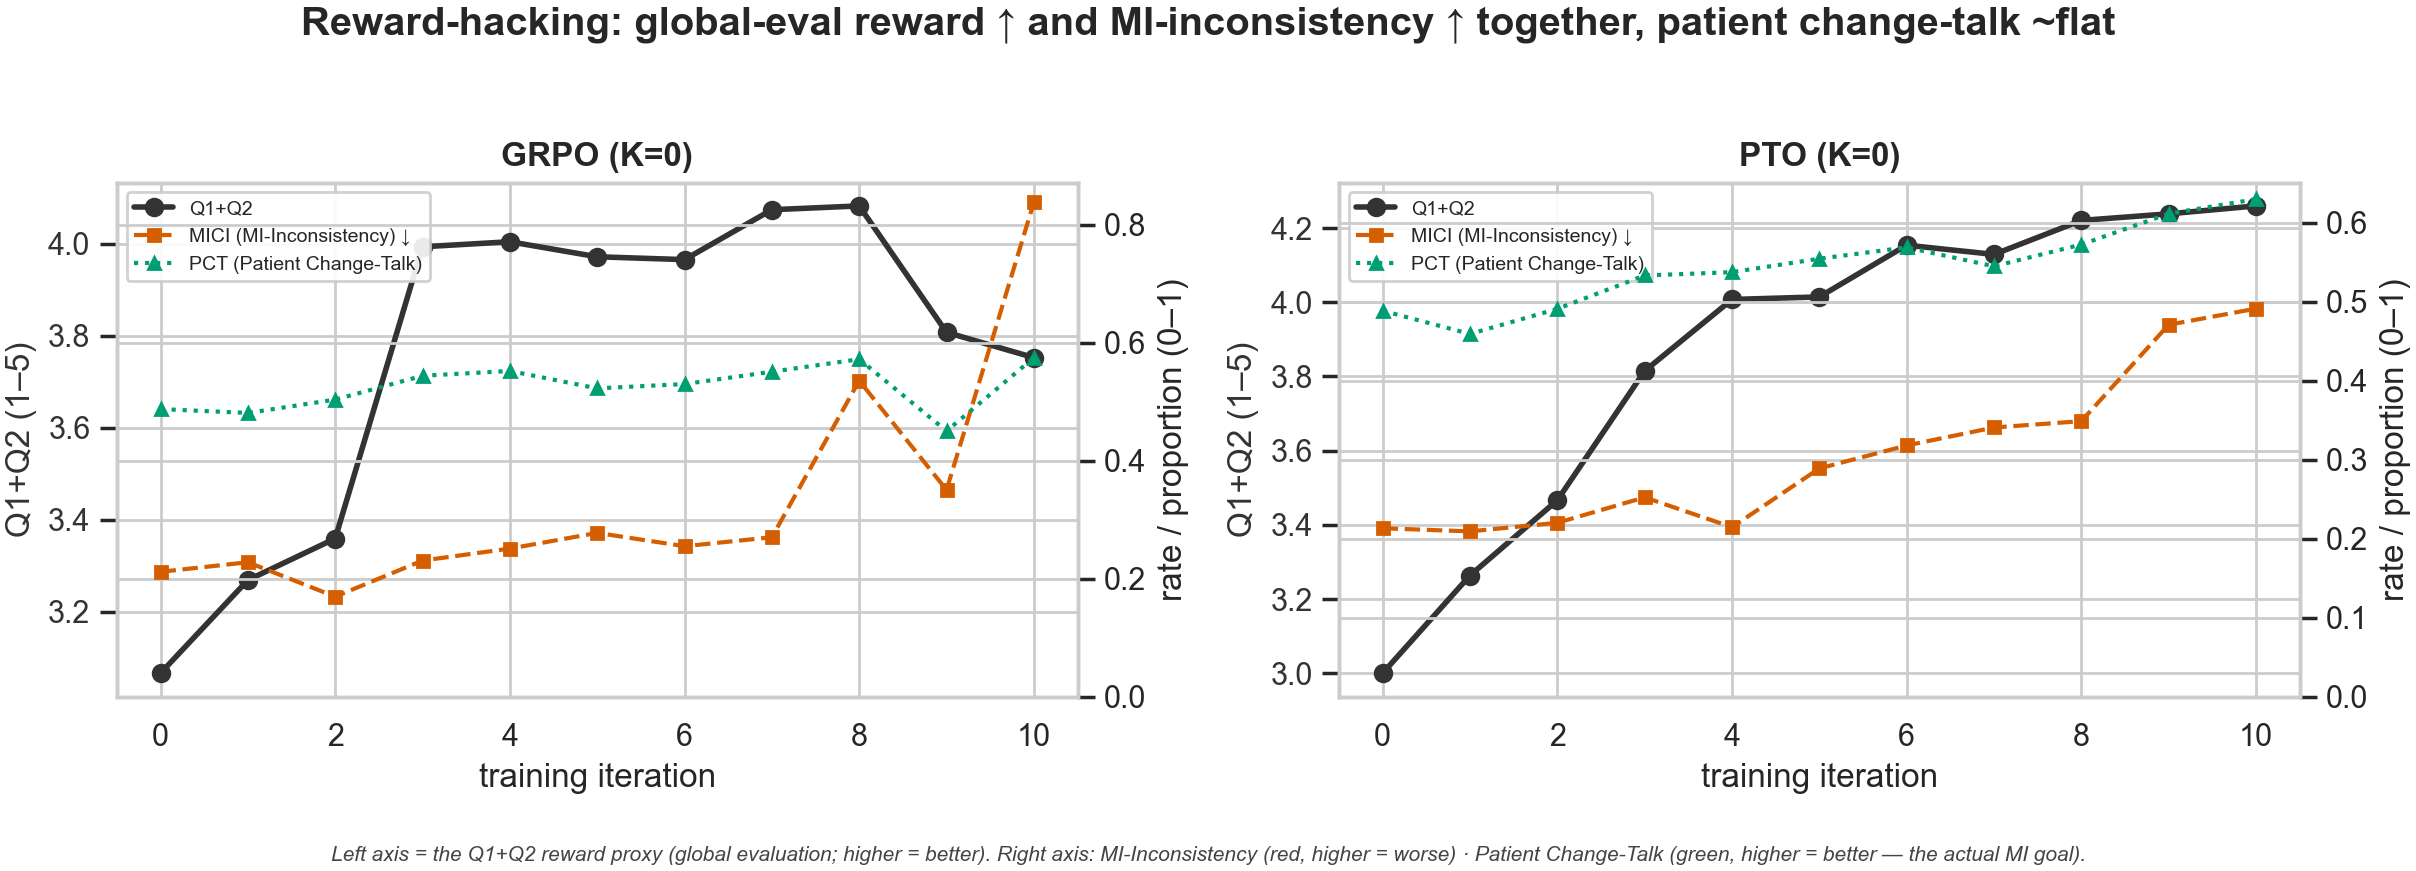
\includegraphics[width=\linewidth]{figures/reward_hack_panel_gpt-4o-mini.png}
  \caption{The reward hack in one frame, per arm. The training reward (\QQ{}, left axis)
  climbs; MI-\emph{inconsistency} (\mici{}, right axis, lower is better) climbs with it;
  patient change-talk (PCT) barely moves. ``All rubrics up'' is not multi-skill improvement.}
  \label{fig:hackpanel}
\end{figure}

The scores in \S\ref{sec:results} are a claim about a therapist only if the therapist got
better at MI. Three lines of evidence say the picture is more complicated, and that the
complication is worse for GRPO.

\paragraph{MI-inconsistency rises with the reward.}
\mici{} counts MI-inconsistent therapist moves --- confronting, unsolicited advice,
over-praise --- per therapist turn. It is outside the training reward, and it moves the
wrong way in both arms: $0.21 \to 0.49$ for PTO (${\sim}2.3\times$) and $0.21 \to 0.84$ for
GRPO (${\sim}4\times$, $\dz{}=1.72$). Patient change-talk, the one metric that asks whether
the \emph{client} moved, rises only modestly ($0.49 \to 0.63$ PTO, $0.49 \to 0.57$ GRPO).
Figure~\ref{fig:hackpanel} puts the three on one frame.

\paragraph{The therapist stops asking and starts praising.}
The behavioural signature is unambiguous and is visible in deterministic text statistics
that use no LLM at all. Affirmations per therapist turn rise ${\sim}5\times$ in both arms
($0.025 \to 0.142$ PTO; $0.029 \to 0.154$ GRPO), while the literal question rate falls from
$0.93 \to 0.55$ per turn in PTO and collapses from $0.83 \to \mathbf{0.15}$ in GRPO.
The oracle's own MITI question counts fall far less steeply
($0.49 \to 0.41$; $0.45 \to 0.32$), and that divergence is itself informative: late-training
turns increasingly carry question \emph{function} --- an invitation to elaborate --- without
question \emph{syntax}, which is the coder's view of a therapist who has replaced inquiry
with affirming statements. A crude lexical praise-marker count puts GRPO at
${\sim}3.5\times$ PTO's rate at iteration~10.

The consequence shows up in the MITI ratios, where it is easy to misread as progress
(Table~\ref{tab:miti}). GRPO's reflection-to-question ratio ``improves'' from $0.70$ to
$1.43$, crossing the manual's basic-competence threshold --- but it does so by shrinking
the denominator. Read against a question rate that fell by $82\%$, a rising R:Q is the
pathology, not the cure.

\begin{table}[t]
  \centering\small
  \setlength{\tabcolsep}{4pt}
  \begin{tabular}{@{}lcccc@{}}
    \toprule
    & \multicolumn{2}{c}{PTO} & \multicolumn{2}{c}{GRPO}\\
    \cmidrule(lr){2-3}\cmidrule(lr){4-5}
    MITI summary & base & @10 & base & @10\\
    \midrule
    R:Q        & 0.61\ding{55} & 0.75\ding{55} & 0.70\ding{55} & 1.43$^{\dagger}$\\
    \%CR       & 0.31\ding{55} & 0.36\ding{55} & 0.30\ding{55} & 0.41$^{\dagger}$\\
    Technical  & 2.92\ding{55} & 3.93$^{\dagger}$ & 3.05$^{\dagger}$ & 3.64$^{\dagger}$\\
    Relational & 3.34\ding{55} & \textbf{4.61}$^{\ddagger}$ & 3.40\ding{55} & \textbf{4.20}$^{\ddagger}$\\
    \bottomrule
  \end{tabular}
  \caption{Against the MITI 4.2.1 manual's suggested competence thresholds
  \citep{moyers2016miti}: \ding{55}~below basic, $^{\dagger}$~``fair'' (basic competence),
  $^{\ddagger}$~``good'' (proficiency). Thresholds are R:Q $1.0/2.0$, \%CR $0.40/0.50$,
  Technical $3.0/4.0$, Relational $3.5/4.0$. Training carries both arms from below basic
  competence to ``good'' on the \emph{relational} globals, while neither reaches ``good'' on
  the \emph{technique} ratios --- and GRPO's ``fair'' R:Q is reached by the pathological
  route (fewer questions). The manual flags these thresholds as expert opinion for
  ${\sim}$20-minute human sessions; we use them as an anchor, not a certification.}
  \label{tab:miti}
\end{table}

\paragraph{The reward's own items point the same way.}
The hack is not purely an optimizer artifact --- some of it is written into the reward. Q2
contributes 17 of the 22 reward items, and the three largest per-item gains at iteration~10
are the same three in both arms: \emph{``revealed what he was thinking''}
($+1.48$ PTO / $+1.07$ GRPO), \emph{``put himself in my shoes''} ($+1.54$ / $+1.01$), and
\emph{``took charge''} ($+1.48$ / $+0.99$). Two of those three reward the therapist for
\emph{self-disclosure} and one for \emph{taking control} --- neither of which MI prescribes,
and the latter of which MI explicitly discourages. An instrument built to measure relational
communication in general dialogue, used as an MI reward, pays for emotive self-revelation.
Optimizers find that.

\paragraph{Reading.}
Both methods buy a real and large improvement in how satisfying and warm the session feels
to a simulated client, together with a real and smaller degradation in MI technique. The
two methods differ in the exchange rate. That framing --- rather than ``PTO is better'' ---
is what we think survives, and the next section gives an independent test of it.

% !TeX root = ../main.tex
\section{Auditing the Judge: Gain Retention}
\label{sec:validity}

Everything so far was graded by the model that supplied the training reward and that also
played the patient. To test whether the conclusions are properties of the therapist or of
that grader, we re-scored the \emph{entire} grid --- every conversation, every rubric, every
model state, $22{,}272$ cells --- with \heldoutjudge{}: a different model family that never
played the patient and never touched training.

\paragraph{The measuring instruments are repeatable.}
Reproducibility is measured rather than assumed. Re-scoring the same conversations with
only the sampling seed changed gives ICC(2,1) \citep{shrout1979icc} of $0.98$--$0.99$ (Q1),
$0.96$--$0.99$ (Q2) and $0.86$--$0.94$ (\mici{}) for the primary oracle, and
$0.95$--$0.98$ / $0.94$--$0.96$ / $0.53$--$0.93$ for the held-out judge
(Appendix~\ref{app:reliability}, Table~\ref{tab:icc}) --- ``excellent'' on the reward
instruments by the \citet{koo2016icc} guideline. This matters for reading the next
paragraph: two noisy raters cannot agree perfectly even if they measure the same thing, so
cross-judge agreement must be read against the attenuation ceiling
$\sqrt{\mathrm{ICC}_a \cdot \mathrm{ICC}_b}$, never against $1.0$
(Table~\ref{tab:ceiling}).

\paragraph{The rankings survive.}
Across all $1{,}848$ pairwise (arm $\times$ metric) contrasts in this comparison, $88.3\%$
keep their sign under the held-out judge, rising monotonically with effect size to $94.1\%$
at $|\Delta|\!\ge\!0.10$, $97.0\%$ at $\ge\!0.25$ and $98.9\%$ at $\ge\!0.50$ (Appendix~\ref{app:signs},
Table~\ref{tab:signladder}): the two
graders disagree only about differences too small to claim. All 18 contrasts this paper
leans on --- including the steelman PTO@10 $-$ GRPO@8 and the regression claim
GRPO@8 $-$ GRPO@10 --- are preserved with bootstrap CIs excluding zero, and the held-out
judge in fact \emph{widens} the headline Q1 gap ($+0.77$ vs the primary's $+0.53$). A
two-way decomposition of the arm means puts only $1.2$--$6.9\%$ of variance in the
arm~$\times$~judge interaction, the only component that could invalidate an ordering; the
judges differ on \emph{level} (the held-out judge is $1.2$--$1.7$ points harsher), which
cancels in every contrast we report.

\paragraph{One rubric genuinely disagrees.}
MITI is the exception and we flag it as a limitation rather than a footnote: only $3.6\%$
of its arm-mean variance is between-arm signal, a single-judge MITI ranking is $0.65$
dependable against ${\approx}0.90$ for every other rubric, and it preserves its sign on only
$77.5\%$ of contrasts --- and, unlike every other rubric, still only $88.2\%$ at
$|\Delta|\!\ge\!0.25$, i.e.\ it can flip at a gap large enough to want to report.
\textbf{MITI arm differences in this paper should be treated as provisional unless both
graders agree on the direction.} \mici{} agrees only weakly per conversation
($r=0.20$--$0.55$); against the measured ceiling it recovers ${\approx}39\%$ of achievable
agreement where Q1/Q2 recover ${\approx}85\%$, so the residual is mostly genuine construct
disagreement about what counts as MI-inconsistent. We therefore state the sycophancy claim
at the \emph{contrast} level (both graders agree GRPO@10 is more MI-inconsistent than
PTO@10, and that \mici{} rises from base in both arms) and not as a precise rate.

\paragraph{Gain retention separates the arms.}
The sharpest use of a held-out grader is not agreement but \emph{retention}. Because the
primary oracle was the training reward and the second judge never touched training,
\[
  \text{retention} \;=\;
  \frac{\Delta_{\text{held-out judge}}}{\Delta_{\text{trained-against judge}}}
\]
is a train/test generalization ratio for each arm's gain over base: ${\approx}1$ means a
behaviour change both graders see, ${\approx}0$ means a gain that existed only inside the
optimized grader. On Q1 the arms separate and their intervals do not overlap:
PTO@10 $0.80\,[0.68, 0.93]$ versus GRPO@10 $0.28\,[0.06, 0.43]$ (GRPO@8:
$0.64\,[0.53, 0.78]$). Under a judge that never graded during training, GRPO's net
ten-iteration Q1 gain is ${\approx}0.19$ points --- close to where it started --- against
the ${\approx}0.68$ the primary grader credits it. Q2 retention, by contrast, is flat at
$0.80$--$0.85$ with fully overlapping intervals, which is ordinary scale compression
between graders and is exactly the null result that makes the Q1 divergence readable as
arm-specific rather than as a grader artifact.

\begin{table}[t]
  \centering\small
  \setlength{\tabcolsep}{3.4pt}
  \begin{tabular}{@{}lcccccccccc@{}}
    \toprule
    iter & 1 & 2 & 3 & 4 & 5 & 6 & 7 & 8 & 9 & 10\\
    \midrule
    PTO  & .97 & .84 & .89 & .94 & .98 & .97 & .94 & .89 & .88 & \textbf{.80}\\
    GRPO & 1.13 & .79 & .89 & .79 & .73 & .57 & .70 & .64 & .03 & \textbf{.28}\\
    \bottomrule
  \end{tabular}
  \caption{Q1 gain retention by iteration. The arms are indistinguishable for three
  iterations, then separate: PTO holds $0.80$--$0.98$ for the whole run while GRPO decays
  monotonically in trend. This is an onset curve, not an endpoint accident.}
  \label{tab:retention}
\end{table}

\begin{figure}[t]
  \centering
  
\includegraphics[width=\linewidth]{figures/multijudge_retention_trajectory.png}
  \caption{Gain retention across iterations (Table~\ref{tab:retention}, plotted). The
  held-out grader stops crediting GRPO's gains \emph{progressively} --- the signature of a
  policy drifting onto grader-specific features rather than of a bad final checkpoint.}
  \label{fig:retention}
\end{figure}

\paragraph{Why this is the load-bearing evidence.}
Retention is measured on Q1 --- an instrument \emph{inside} the training reward --- which
makes it immune to the objection that outside-the-reward instruments (\mici{}, MITI) might
simply be measuring something the training never targeted. It requires no human coding, no
new conversations, and one extra grading pass. And it is an onset curve
(Table~\ref{tab:retention}, Figure~\ref{fig:retention}): the divergence begins at
iteration~3 and grows, which is what optimizer drift looks like and is not what a single
bad checkpoint looks like. We propose it as a default diagnostic for any system trained
against an LLM judge: \emph{report how much of your gain a grader that never saw training
still credits, per iteration.}

% !TeX root = ../main.tex
\section{Where the Difference Comes From}
\label{sec:mechanism}

The two arms differ in a loss \emph{and} in a data-collection strategy. Which carries the
gap? Preference turns out not to be the essential difference: both methods weight the
candidates of a group and step along the weighted sum --- DPO puts $+1$ on the logged winner
and $-1$ on the loser, GRPO the standardized advantage on each of its $G$ completions ---
so rescaling every group's weights to a common size puts both on one probe and lets us read
the training signal directly. Appendix~\ref{app:mechanism} gives the construction, the probe
audit that disqualifies per-iteration estimates, and the per-iteration series; two results
matter here.

\paragraph{The reward hack is visible in the gradient, and it compounds.}
The update's affirmation push --- exact, embedding-free, over every group --- rises from
$-0.006$ to $+0.086$ in GRPO and from $0.008$ to $0.103$ in PTO, so \S\ref{sec:hacking}'s
drift has a training-side measurement and not only an outcome-side inference. But that
selection pressure is an order of magnitude smaller than the drift it produces: over all
sampled candidates, affirmation cues go $0.02 \to 0.54$ (GRPO) and question marks
$0.71 \to 0.06$. Small, same-signed pressure applied each iteration to an
already-more-effusive policy compounds --- which matters for mitigation, since penalising the
selection step would barely touch a drift that lives in the generation distribution.

\paragraph{The gap is the data, not the loss.}
The arms' pooled update directions agree only weakly (cosine $0.32$, corrected for how well
each is estimated). Applying each method's weighting rule to the \emph{other's} candidate
groups isolates why:

\begin{center}\small
\begin{tabular}{@{}lr@{}}
\toprule
Comparison & cos\\
\midrule
As trained (rule \emph{and} data differ) & 0.32\\
Same groups, rule swapped (PTO's data)   & 0.91\\
Same groups, rule swapped (GRPO's data)  & 0.99\\
Same rule, each method's own data        & 0.40 / 0.32\\
\bottomrule
\end{tabular}
\end{center}

\noindent
Swapping the rule on identical groups barely moves the update; holding the rule fixed and
swapping the groups leaves the arms as far apart as when trained. \textbf{At matched $K$ and
a shared oracle, DPO and group-relative weighting extract nearly the same direction from the
same eight completions.} ``PTO vs GRPO'' is therefore a statement about \emph{exploration}
--- which conversational states each method collects candidates in --- not about the loss
family, and the design question becomes which states to visit rather than which objective to
use. One caution on our own headline: PTO's $\tau$ filter and shrinking branch count cost it
two-thirds of its training signal over the run (groups trained $782 \to 281$, against
$94$--$98\%$ retention for GRPO), so a flattening PTO curve may partly be a data-starvation
curve (Appendix~\ref{app:mechanism}, Table~\ref{tab:yield}).

% !TeX root = ../main.tex
\section{Discussion}
\label{sec:discussion}

\paragraph{What a practitioner should take from this.}
If you are training a small model to do MI against an LLM oracle, three things follow.
(i)~\textbf{Do not stop at the reward curve.} Both arms here would report a large, highly
significant, multi-rubric success, and one of them ends with a therapist that asks a
question every seventh turn. (ii)~\textbf{Buy a second grader before you buy more
iterations.} Re-scoring the whole grid with a held-out judge cost less than a single
training iteration and is what separated a real gain from a grader-specific one. (iii)~
\textbf{Prefer the method that explores}, and treat iteration count as a hyperparameter with
a validation criterion attached --- GRPO's best model is four iterations before its last.

\paragraph{Why the winner wins.}
Our reading is that PTO's advantage is not the DPO loss (\S\ref{sec:mechanism} rules that
out fairly directly) but the sequential trunk. Because each branch point commits to its
winner and continues, PTO collects candidates in states reached by a run of good choices ---
states that GRPO's fixed, once-per-iteration prompt list never contains. That is a
distribution-of-training-contexts advantage, and it also predicts the observed cost: PTO's
sequential growth cannot be batched as freely, and its $\tau$ filter throws data away.

\paragraph{Why the loser loses in a specific way.}
GRPO's failure is not instability in the usual RL sense --- it improves monotonically for
eight iterations and its variance is unremarkable. It fails by \emph{succeeding at the
stated objective}: it drives the reward up, and the reward is a 22-item questionnaire in
which self-disclosure and taking charge are credited. The clinical failure mode
(a warm, praising, non-inquiring counsellor) and the machine-learning failure mode (a policy
overfitting its grader) turn out to be the same event viewed from two instruments, which is
what makes MI a good testbed for reward hacking rather than merely a domain in which it
occurs.

\paragraph{On the instruments.}
The most uncomfortable finding for the paradigm is \S\ref{sec:results}'s factor structure:
five rubrics that sound like five constructs behave like one. A study that reports Q1, Q2,
WAI-SR, CSQ-8 and MI-SAT all improving has, to a first approximation, reported one number
five times. Batteries for LLM-graded MI should be chosen for what they \emph{dis}agree
about --- which, empirically here, means MI-inconsistency counts and the MITI technique
ratios --- and not for how many validated instruments they contain.

\section{Conclusion}
\label{sec:conclusion}

We compared preference-tree and group-relative optimization for training a 1B therapist
model to do Motivational Interviewing, holding the base policy, the simulated patients, the
grading oracle, the candidate budget and the look-ahead depth fixed. Both raise the reward
substantially; PTO leads at the matched ten-iteration endpoint and keeps improving where
GRPO peaks and regresses. But the gains in both arms come with a drift toward affirmation
and away from inquiry, and a judge that never touched training credits $0.80$ of PTO's Q1
gain against $0.28$ of GRPO's --- an onset curve that begins at iteration~3. Reading the
training signal directly shows the two losses extract nearly the same direction from the
same candidates, so the method gap is about which conversational states get explored, not
about DPO versus group-relative weighting. We recommend gain retention under a decoupled
grader as a routine diagnostic wherever an LLM fills in a questionnaire for reward.

% !TeX root = ../main.tex
\section*{Limitations}
\label{sec:limitations}

\paragraph{No human MI coding.}
Every number here comes from an LLM. Both graders' repeatability is measured
(\S\ref{sec:validity}), but an oracle can be perfectly repeatable and consistently wrong; a
grader that never touched training bounds \emph{shared-target} bias, not \emph{shared-model}
bias. A human-coded sample --- particularly of \mici{}, where the two graders agree least
--- remains the strongest available addition and is the obvious next step.

\paragraph{The generator is not decoupled, only the grader.}
The patient simulator is \texttt{gpt-4o-mini} in every conversation of both arms. The second
judge decouples \emph{evaluation} from the training reward; it does not decouple the
environment. A fully decoupled replication would require re-simulating every conversation
with a patient from another model family.

\paragraph{Circularity in the headline metric.}
\QQ{} is both the training reward and a reported outcome, so ``\QQ{} improved'' cannot by
itself demonstrate MI skill. We mitigate rather than remove this: the outside-the-reward
axes (\mici{}, PCT, the MITI ratios) and the deterministic text statistics carry the
reward-hacking argument, and gain retention converts the circularity into a measured
train/test ratio. \QQ{} is best read as a satisfaction/alliance proxy.

\paragraph{MITI differences are provisional.}
MITI has the weakest cross-grader behaviour of the eight instruments (dependability $0.65$
from one judge; sign preserved on $77.5\%$ of contrasts, and only $88.2\%$ even at
$|\Delta|\!\ge\!0.25$). Table~\ref{tab:miti}'s threshold verdicts should be read as
indicative. \mici{} agrees weakly per conversation, which is why its claims are stated as
contrasts and never as rates.

\paragraph{One seed, one base model, one look-ahead setting.}
Each arm is a single ten-iteration run of a single 1B base policy at $K = 0$. Persona-paired
tests control the evaluation variance ($n = 96$ per cell) but not run-to-run training
variance; replicate seeds were outside the compute and API budget. Whether the same ordering
holds at larger policy scale, at $K > 0$, or under a different reward composition is open ---
$K$ is the subject of a companion study.

\paragraph{Multiplicity.}
Holm/BH corrections are applied \emph{within} families (the rubrics of one contrast, or the
iterations of one arm-vs-base sweep) and are not pooled across the families in the paper.
We treat the endpoint PTO-vs-GRPO contrast and the arm-vs-base sweeps as confirmatory, and
everything in \S\ref{sec:hacking} and \S\ref{sec:mechanism} as descriptive.

\paragraph{Simulated patients are not patients.}
The 96 personas are a factorial over six attributes and two presenting problems, written to
be tractable rather than representative. Nothing here licenses a claim about how these
models would behave with a person.

% !TeX root = ../main.tex
\section*{Ethical Considerations}

The system studied here is a research artifact. \textbf{It is not a therapeutic tool and
must not be deployed with people in distress}, and this paper's central finding is a reason
to say so more strongly rather than less: an MI agent optimized against an LLM-filled
questionnaire can score highly \emph{because} it praises the client and stops asking
questions --- behaviour that reads as supportive, is measurably MI-inconsistent, and would
be actively unhelpful to someone ambivalent about change. A system optimized against
patient-perspective satisfaction has a structural incentive toward telling users what they
want to hear; in a mental-health context that is a safety property, not a style preference.
We would go further: the gain-retention gap in \S\ref{sec:validity} shows the drift is
invisible to the very instrument used to certify progress, so an evaluation pipeline built
from a single LLM grader should not be treated as a safety check.

No human subjects were involved and no personal data was used; all conversations are
synthetic, generated between two language models. The simulated personas cover two
health-behaviour problems (smoking, obesity) with fixed demographic attributes. Obesity in
particular is a domain in which careless framing causes real harm, and the persona prompts
were not reviewed by clinicians for stigmatising content --- a gap we name rather than
excuse. Model outputs were not safety-filtered before scoring.

The therapist model is used under the Llama Community License. Both graders are commercial
APIs, so a study whose measuring instrument is a served proprietary checkpoint is
reproducible only for as long as that checkpoint is served; we mitigate this by releasing
all scored conversations and per-conversation scores rather than only aggregate results.
\todo{confirm the release plan --- conversations + score lake + code? decide before
submission.} Compute and API costs are reported in Appendix~\ref{app:cost}.


\bibliography{refs}

\appendix
% !TeX root = ../main.tex
\section{Judge Reliability in Full}
\label{app:reliability}

Repeatability is estimated as ICC(2,1) (two-way random effects, absolute agreement, single
rater) across re-scorings of the same conversations differing only in the API sampling seed,
on an anchor subset of four model states $\times$ $96$ conversations. The primary oracle's
estimate spans four draws (three seeded reps plus the draw the paper reports); the held-out
judge's spans three.

\begin{table}[h]
  \centering\small
  \begin{tabular}{@{}lcc@{}}
    \toprule
    & \multicolumn{2}{c}{ICC(2,1)}\\
    \cmidrule(lr){2-3}
    Metric & primary & held-out judge\\
    \midrule
    Q1     & 0.982--0.994 & 0.951--0.978\\
    Q2     & 0.955--0.992 & 0.938--0.963\\
    \mici{} & 0.864--0.943 & 0.525--0.929\\
    \bottomrule
  \end{tabular}
  \caption{Both graders are highly repeatable on the reward instruments. The held-out
  judge's \mici{} repeatability \emph{falls as the MI-inconsistency rate rises} (0.93 at the
  base policy, 0.53 at GRPO@10), i.e.\ it is least reliable exactly where the sycophancy
  claim lives --- which is why \S\ref{sec:validity} states that claim at the contrast level.}
  \label{tab:icc}
\end{table}

\begin{table}[h]
  \centering\small
  \begin{tabular}{@{}lccc@{}}
    \toprule
    Metric & observed $r$ & ceiling & \% of ceiling\\
    \midrule
    Q1      & 0.84--0.88 & 0.97--0.99 & 86--91\%\\
    Q2      & 0.80--0.86 & 0.96--0.98 & 83--88\%\\
    \mici{} & 0.20--0.55 & 0.70--0.93 & \textbf{29--59\%}\\
    \bottomrule
  \end{tabular}
  \caption{Per-conversation cross-grader agreement against the attenuation ceiling
  $\sqrt{\mathrm{ICC}_a\cdot\mathrm{ICC}_b}$, both terms measured. Q1 and Q2 recover most of
  the achievable agreement; \mici{} does not, and the residual is construct disagreement
  about what counts as MI-inconsistent, not merely noise.}
  \label{tab:ceiling}
\end{table}

\section{Sign Preservation Ladder}
\label{app:signs}

Every pairwise (model state $\times$ metric) contrast in the comparison --- $1{,}848$ of
them --- re-computed under the held-out grader and checked for sign agreement, laddered by
the size of the difference the primary grader reports.

\begin{table}[h]
  \centering\small
  \begin{tabular}{@{}lcc@{}}
    \toprule
    Contrast set & $n$ & sign preserved\\
    \midrule
    all                      & 1848 & 88.3\%\\
    $|\Delta| \ge 0.10$      & --   & 94.1\%\\
    $|\Delta| \ge 0.25$      & --   & 97.0\%\\
    $|\Delta| \ge 0.50$      & --   & 98.9\%\\
    \midrule
    MITI only, all           & --   & 77.5\%\\
    MITI only, $\ge 0.25$    & --   & 88.2\%\\
    \bottomrule
  \end{tabular}
  \caption{Agreement rises monotonically with effect size: the graders disagree only about
  differences too small to claim --- except on MITI, which still disagrees at claimable
  gaps. \todo{fill per-row $n$ from
  \texttt{multijudge\_sign\_\-preservation.md}.} Thresholds are
  absolute, so read a ladder down its own rubric and not across rubrics (PCT and \mici{}
  live on $[0,1]$; the Likert rubrics on $1$--$5$).}
  \label{tab:signladder}
\end{table}

\section{Cost}
\label{app:cost}

Training ran on a single A100 (Colab) for both arms; evaluation and scoring ran locally
against commercial APIs. Grading cost is dominated by call \emph{count}
(model states $\times$ rubrics $\times$ conversations), and the oracle prompt is laid out
rubric-first so that its fixed prefix is prompt-cached.

\begin{itemize}\itemsep1pt
  \item Primary oracle (training reward + full evaluation grid, both arms):
        \todo{split the project's ${\approx}\$300$ OpenAI total into the K=0 share for this
        paper --- the rest belongs to the companion look-ahead study.}
  \item Held-out judge, full $22{,}272$-cell sweep: \$42 (Anthropic Message Batches, 50\%
        discount; measured $3{,}621$ input $+$ $71$ output tokens per call).
  \item Held-out judge repeatability reps (Appendix~\ref{app:reliability}): \$9.16.
  \item GPU: \todo{report A100-hours per arm from the run metadata.}
\end{itemize}

A design note worth stating, since it is the choice most likely to be questioned: the
held-out sweep was run at \textbf{one} repetition per cell rather than three. Grader
sampling noise contributes ${\approx}0.01$ to a 96-conversation arm mean against
${\approx}0.09$ from persona sampling, so at equal cost breadth (all model states) strictly
dominates depth (more reps of a few). Depth was bought only where breadth could not answer
the question --- the held-out judge's own repeatability, without which weak \mici{}
agreement is uninterpretable.

\section{Reproducibility}
\label{app:repro}

\todo{Fill before submission: repository URL, the exact commit, adapter checkpoints on the
Hub, and the released score files. Note the analysis is seeded (bootstrap seed fixed) and
figures regenerate from the tracked artifacts.}

% !TeX root = ../main.tex
\section{Reading the Training Signal: Full Construction and Results}
\label{app:mechanism}

This appendix expands \S\ref{sec:mechanism}. It measures what each method's update pushes
toward, from the training data itself rather than from outcomes.

\subsection{Putting two losses on one probe}

Both methods weight the candidates of a group and step along the weighted sum. For a group
of candidates $\{y_g\}$ each is assigned a weight $w_g$:

\begin{itemize}\itemsep2pt
  \item \textbf{PTO / DPO:} $w_g = +1$ on the logged \emph{chosen}, $-1$ on
  \emph{rejected}, $0$ otherwise --- i.e.\ the literal $\tau$-filtered pair.
  \item \textbf{GRPO:} $w_g = (r_g - \mathrm{mean}_g\,r)/\mathrm{std}_g\,r$, the
  standardized advantage that scales each completion's gradient.
\end{itemize}

\noindent
Weights are then rescaled \emph{within each group} to $\sum_g |w_g| = 2$, which is DPO's
natural scale. This rescaling is what makes the two comparable: without it, GRPO's weights
carry the group's reward spread and every cross-method quantity becomes a scale artifact.
Groups lacking either sign are dropped --- for PTO that means a branch point the $\tau$
filter left unpaired, which never trained.

Two readouts are taken off the weighted groups:

\begin{itemize}\itemsep2pt
  \item \textbf{Lexical push} $\sum_g w_g\,\phi(y_g)$, averaged over groups with a standard
  error, for a feature $\phi \in \{$length, question marks, affirmation cues, over-praise
  cues$\}$. Units are chosen-minus-rejected, so $0$ means the update is indifferent to the
  feature. This is exact, uses no embeddings, and covers every group. The affirmation and
  over-praise cue sets are deliberately the \emph{same} regexes used for the
  conversation-side checks in \S\ref{sec:hacking}, so the two sides are able to agree.
  \item \textbf{Update direction} $\mathrm{normalize}(\sum_g w_g\, e(y_g))$ in sentence-
  embedding space --- a mass-mean probe generalized to an arbitrary weighting.
\end{itemize}

\paragraph{A probe audit, and what it disqualifies.}
Directions are only usable where they are actually estimated. Scoring each half of an
iteration's groups with the other half's direction gives a split-half reliability of
$0.15$--$0.32$ for a \emph{per-iteration} PTO direction --- two halves of one iteration point
almost independently --- so per-iteration direction results are estimation noise and we do
not report them. Pooled over iterations the directions are usable ($0.60$ PTO, $0.91$ GRPO),
and all direction results below are pooled. Cross-arm cosines are additionally divided by the
attenuation ceiling $\sqrt{r_a r_b}$, since two noisy estimates cannot agree perfectly even
if identical. (For the same-groups rows of Table~\ref{tab:decomp} the correction
over-corrects, because both directions share their estimation noise; a corrected value above
$1.0$ is the tell, so those rows are read raw.)

\subsection{The affirmation push, per iteration}

\begin{figure}[h]
  \centering
  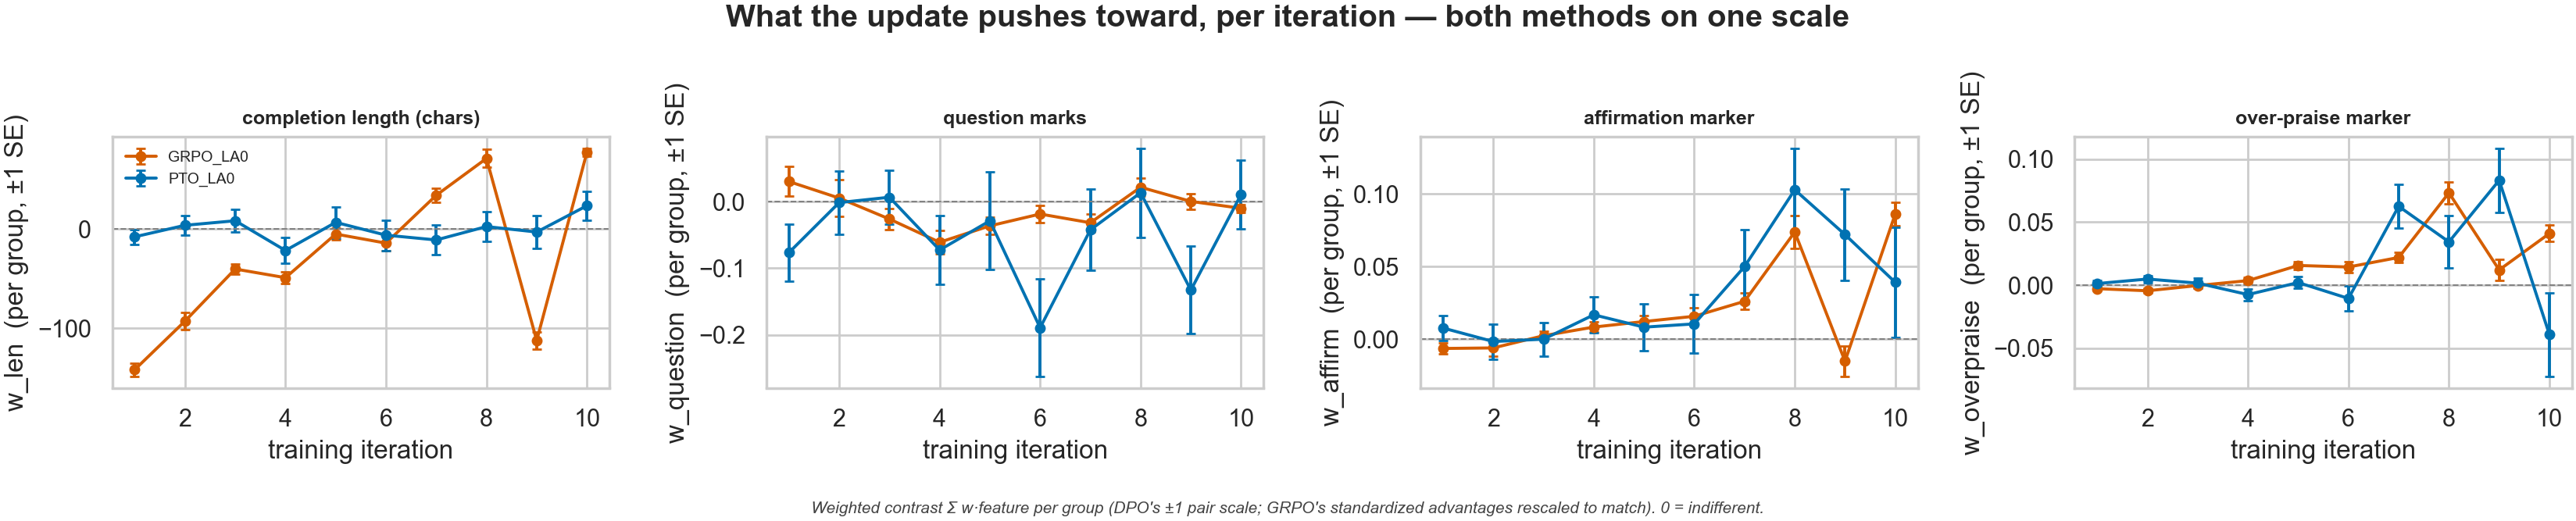
\includegraphics[width=\linewidth]{figures/update_lexical_push_gpt-4o-mini.png}
  \caption{Weighted affirmation contrast per training iteration, $\pm$ SE. Both arms rise;
  GRPO reaches $+0.086\,(\pm0.008)$ at iteration~10 and PTO peaks at $0.103\,(\pm0.029)$ at
  iteration~8 (its iteration-10 estimate, $0.039 \pm 0.038$, rests on far fewer groups --- see
  Table~\ref{tab:yield}). GRPO's series dips \emph{negative} at iteration~9, the same
  iteration at which the outcome grid dips (\S\ref{sec:results}), from a completely
  independent source.}
  \label{fig:push}
\end{figure}

\subsection{Generation versus selection}

\begin{figure}[h]
  \centering
  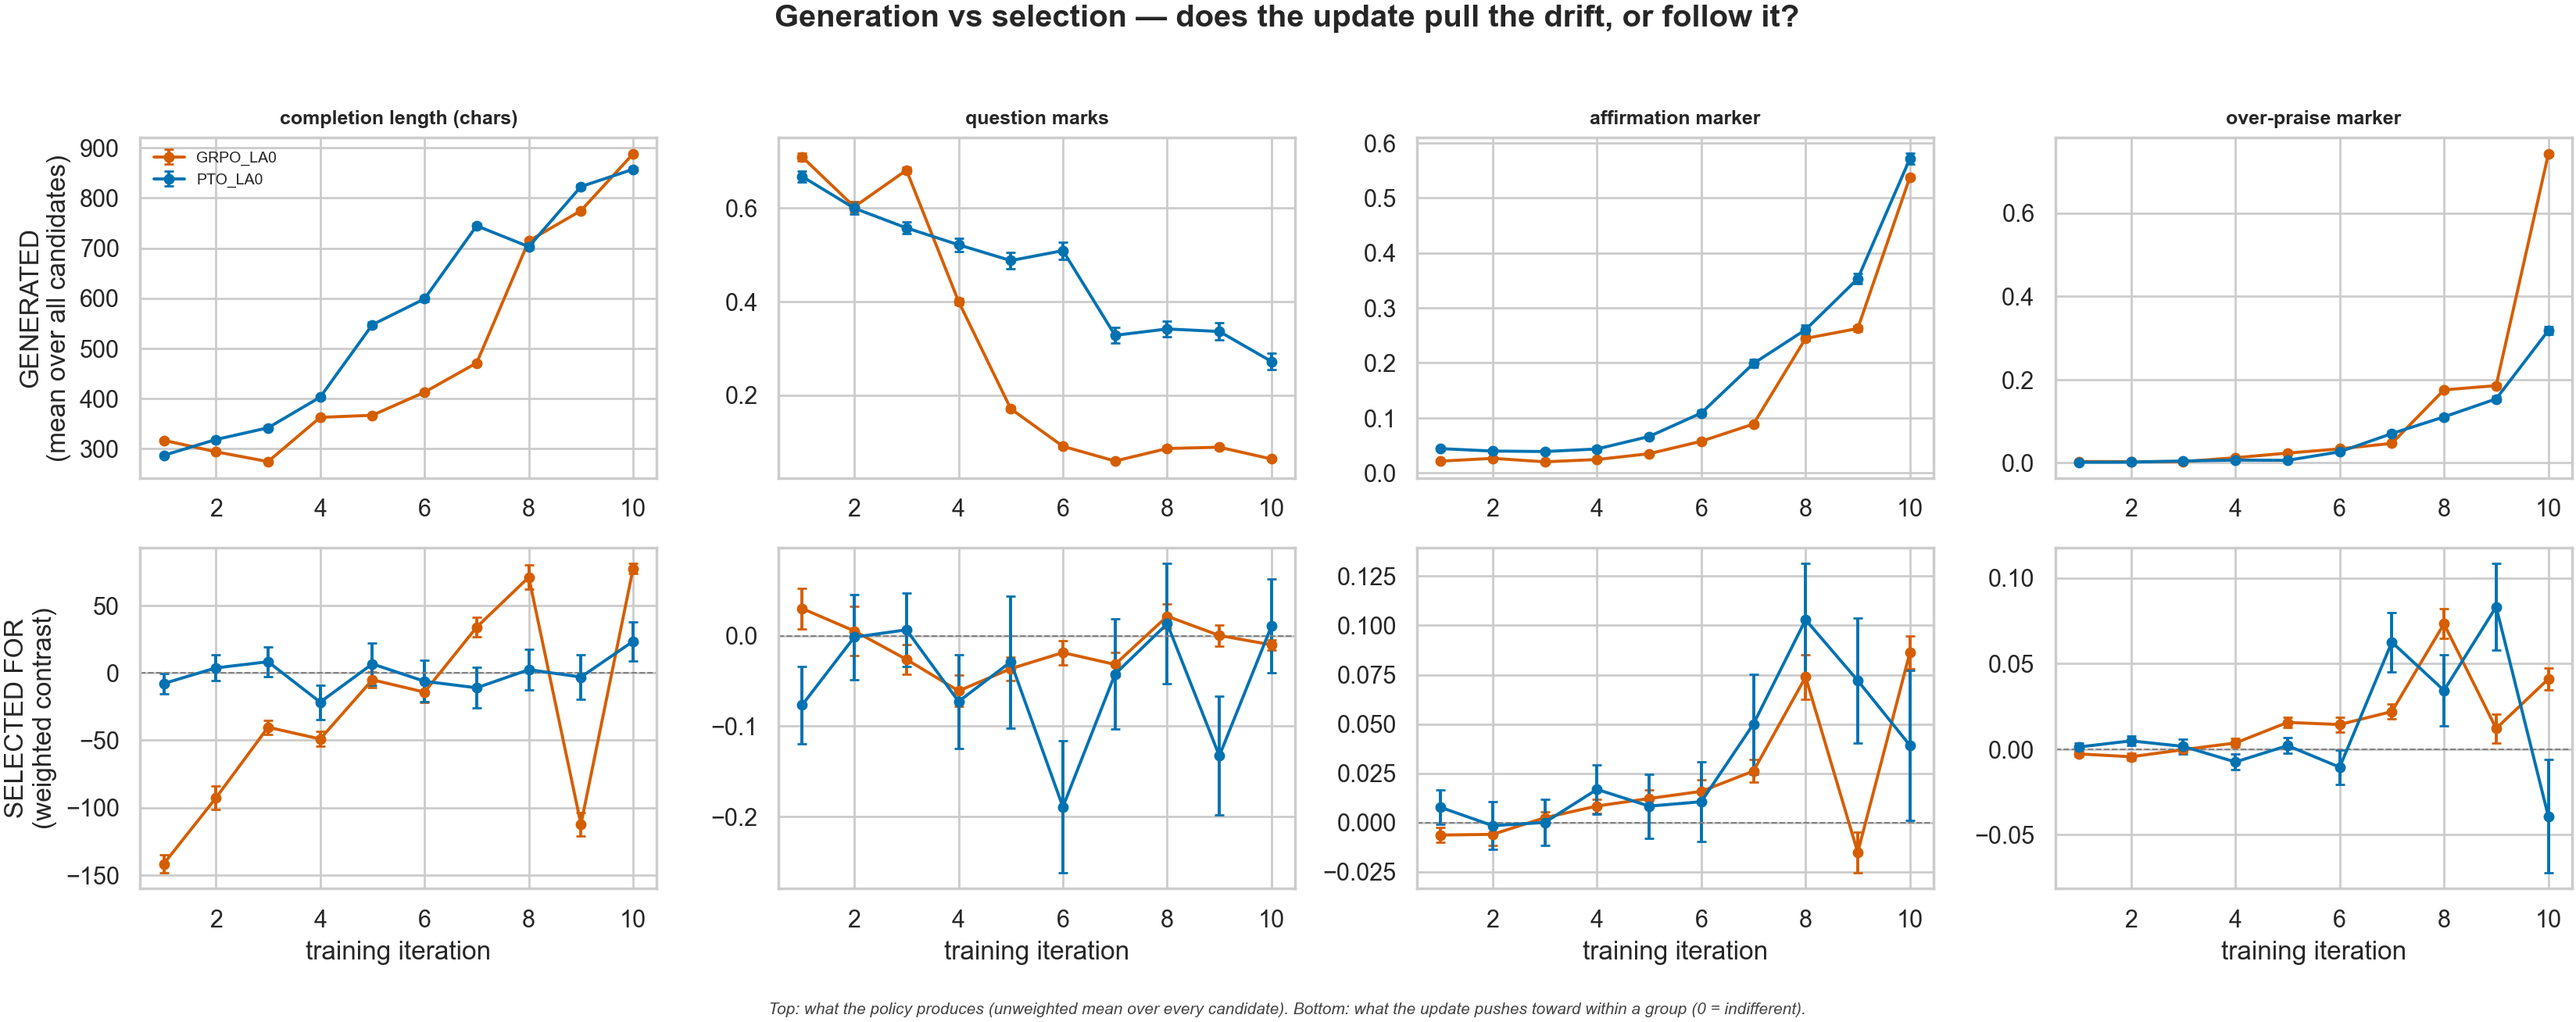
\includegraphics[width=\linewidth]{figures/generation_vs_selection_gpt-4o-mini.png}
  \caption{What the update \emph{selects for} (per-group weighted contrast) against what the
  policy \emph{generates} (unweighted mean over all sampled candidates). The pool moves an
  order of magnitude more than the selection pressure that produces it.}
  \label{fig:genvssel}
\end{figure}

Over all sampled candidates, mean affirmation-cue rate goes $0.021 \to 0.538$ (GRPO) and
$0.044 \to 0.571$ (PTO); over-praise cues reach $0.741$ of GRPO's candidates (PTO $0.318$);
question marks per candidate fall $0.710 \to 0.063$ (GRPO) and $0.668 \to 0.272$ (PTO).
Against a per-iteration selection pressure of ${\approx}0.01$--$0.10$, this is a compounding
on-policy loop rather than one strong pull.

\emph{Indexing note.} Training iteration $n$ samples from the iteration-start policy, so a
pool row describes the policy the evaluation set calls \texttt{model\_iter\_}$(n{-}1)$ ---
deliberately off by one from the selection contrast on the same row.

\subsection{Loss versus data}

\begin{table}[h]
  \centering\small
  \setlength{\tabcolsep}{4pt}
  \begin{tabular}{@{}lccc@{}}
    \toprule
    Comparison & cos & ceil. & corr.\\
    \midrule
    As trained (rule + data differ) & 0.267 & 0.844 & \textbf{0.317}\\
    Same groups (PTO), rule swap    & \textbf{0.908} & --- & ---\\
    Same groups (GRPO), rule swap   & \textbf{0.988} & --- & ---\\
    Same rule (group-rel.), data differ & 0.356 & 0.896 & 0.397\\
    Same rule (best-worst), data differ & 0.266 & 0.823 & 0.324\\
    \bottomrule
  \end{tabular}
  \caption{Decomposing the cross-method update-direction gap by applying each weighting rule
  to the other method's candidate groups. The rule contributes almost nothing; the data
  contributes almost everything. Same-groups rows are read raw (see the audit above).}
  \label{tab:decomp}
\end{table}

\subsection{Training-signal yield}

\begin{table}[h]
  \centering\small
  \begin{tabular}{@{}lrrrr@{}}
    \toprule
    & \multicolumn{2}{c}{PTO} & \multicolumn{2}{c}{GRPO}\\
    \cmidrule(lr){2-3}\cmidrule(lr){4-5}
    Iter & built & trained & built & trained\\
    \midrule
    1  & 949 & 782 & 1728 & 1660\\
    5  & 600 & 483 & 1888 & 1789\\
    10 & 410 & 281 & 2528 & 2484\\
    \midrule
    yield & \multicolumn{2}{c}{$0.82 \to 0.69$} & \multicolumn{2}{c}{$0.94$--$0.98$}\\
    margin & \multicolumn{2}{c}{$0.274 \to 0.196$} & \multicolumn{2}{c}{$0.379 \to 0.339$}\\
    \bottomrule
  \end{tabular}
  \caption{PTO's $\tau$ filter and its shrinking branch count cost it two-thirds of its
  training signal over the run, while GRPO trains on nearly every group it builds. A
  flattening PTO curve may partly be a data-starvation curve. Full per-iteration values in
  the released tables.}
  \label{tab:yield}
\end{table}

\subsection{Does the training push predict the outcome move?}

With the iteration index partialled out of both sides --- mandatory, since both the push
features and the evaluation deltas trend with training by construction --- GRPO's
per-iteration change in \mici{} tracks its affirmation push at $\rho = 0.647$ ($p = .043$),
its length push at $0.706$ ($p = .023$) and its over-praise push at $0.617$ ($p = .057$).
PTO's does not ($-0.492$, n.s.). This is the same direction as the endpoint \mici{} gap
(\S\ref{sec:hacking}), reached from the training data instead of from the transcripts. With
$n \le 10$ iterations per arm and no multiplicity correction it is a mechanism consistent
with the curves, not a demonstrated cause.


\end{document}
